\chapter{Obiekt symulowany - część projektowa}
Pierwszym etapem naszej pracy była analiza dostarczonego przez prowadzącego programu symulującego działanie obiektu. Był to obiekt dyskretny z opóźnieniem zależny od zmiennych procesu $U(k-11)$, $U(k-10)$, $Y(k-1)$, $Y(k-2)$.

Program do obsługi całego zadania symulacji został zaimplementowany w pliku \texttt{Projekt1.m}. Wykonywane są w nim wszystkie wymagane polecenia niezbędne do wykonania zadania, tj. sprawdzenie poprawności wartości w punkcie pracy $U_{\mathrm{pp}}$ i $Y_{\mathrm{pp}}$, wyznaczenie odpowiedzi skokowych procesu, wywołanie funkcji implementujących algorytmy PID i DMC, a także optymalizacja wskaźnika jakości regulacji $E$.

\section{Wyznaczenie odpowiedzi skokowych procesu}
Rozpoczynając od punktu pracy $U_{\mathrm{pp}}=\num{0,8}$ i $Y_{\mathrm{pp}}=2$ wyznaczaliśmy różne odpowiedzi skokowe dla kilku zmian sygnału sterującego. Wyniki symulacji przedstawione są na Rys.~\ref{os}. Jak widać, symulowany obiekt jest stabilny (charakterystyki po pewnym czasie ustalają się na stałym poziomie) oraz liniowy (charakterystyki statyczne $Y(U)$ leżą w przybliżeniu na linii prostej, co przedstawione jest na Rys.~\ref{char_stat}).

Na podstawie tej charakterystyki możemy obliczyć wzmocnienie statyczne procesu. Definiuje się je jako
\begin{equation}
K=\frac{\Delta Y}{\Delta U}
\end{equation}
Parametry $\Delta Y$ i $\Delta U$ są stałe dla dowolnie wybranych punktów na wykresie $Y(U)$, ponieważ charakterystyka jest liniowa. Należy więc wybrać dowolne punkty $(U_i, Y_i)$ i $(U_j, Y_j)$ i na ich podstawie obliczyć wzmocnienie statyczne $K$. Wynik:
\begin{equation}
K=1
\end{equation}

\begin{figure}
\label{os}
\centering
\caption{Odpowiedzi skokowe dla procesu symulowanego}
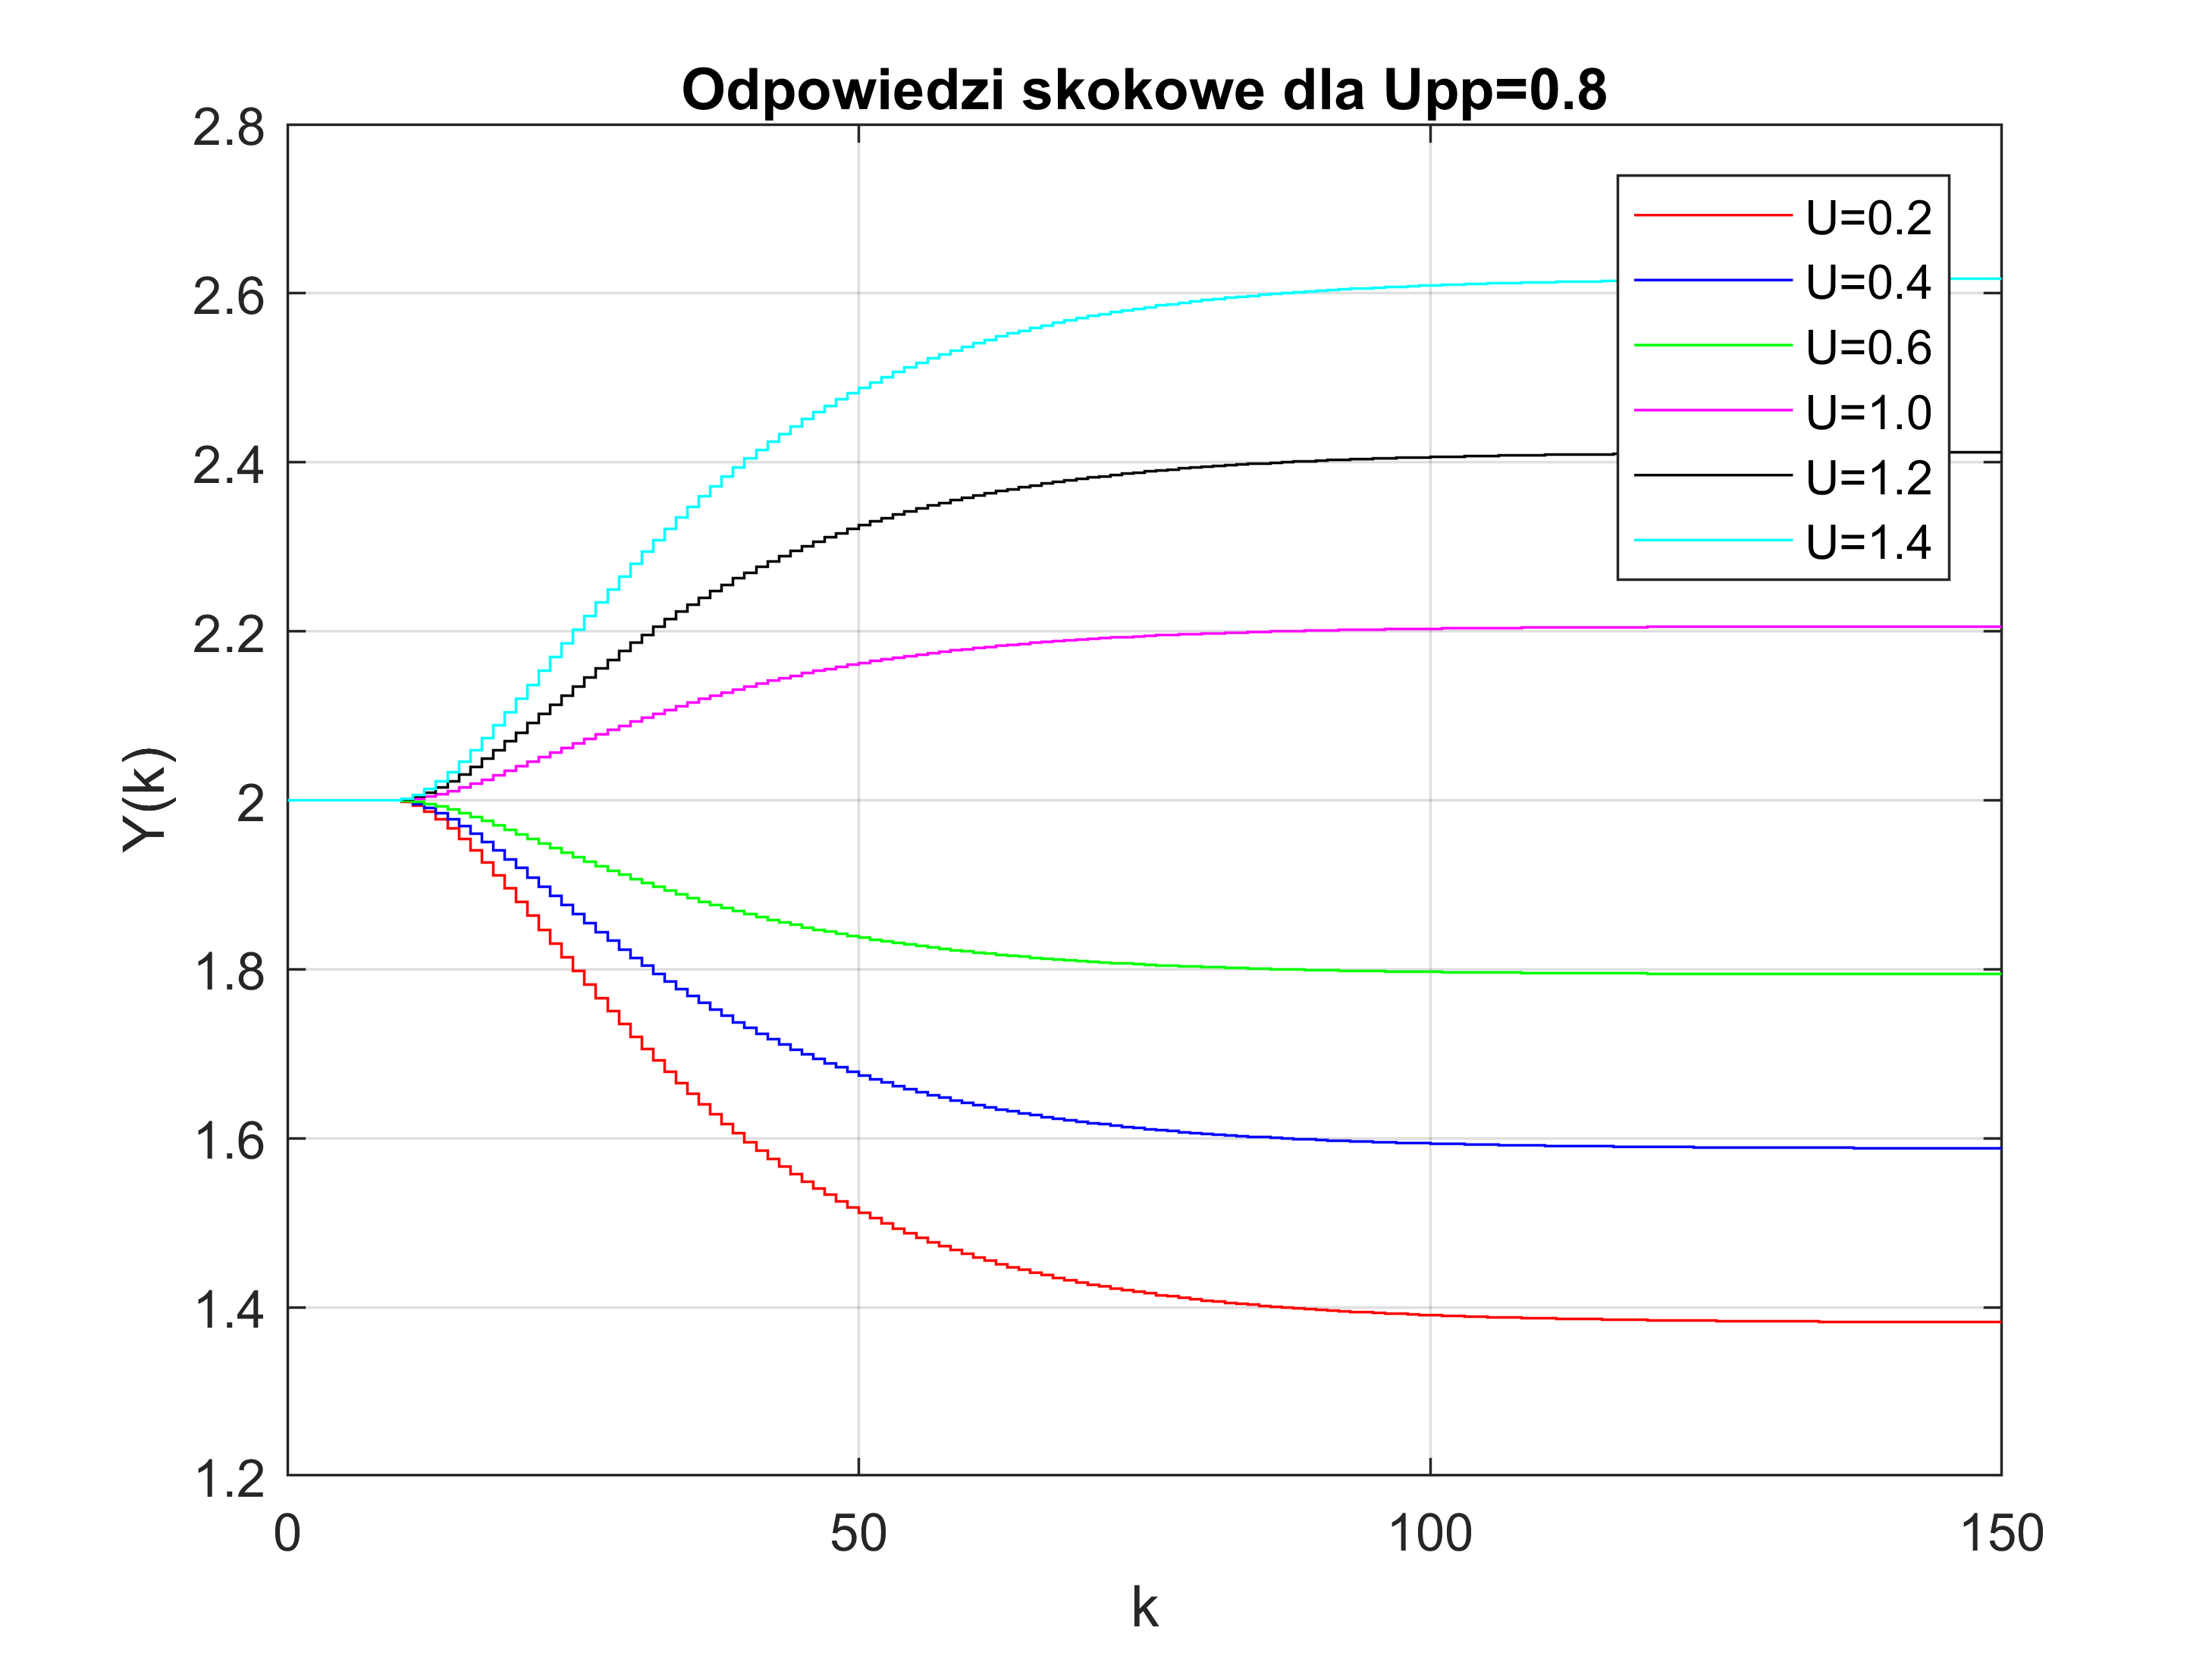
\includegraphics{odpsk.png}
\end{figure}

\begin{figure}
\label{char_stat}
\centering
\caption{Charakterystyki statyczne $Y(U)$}
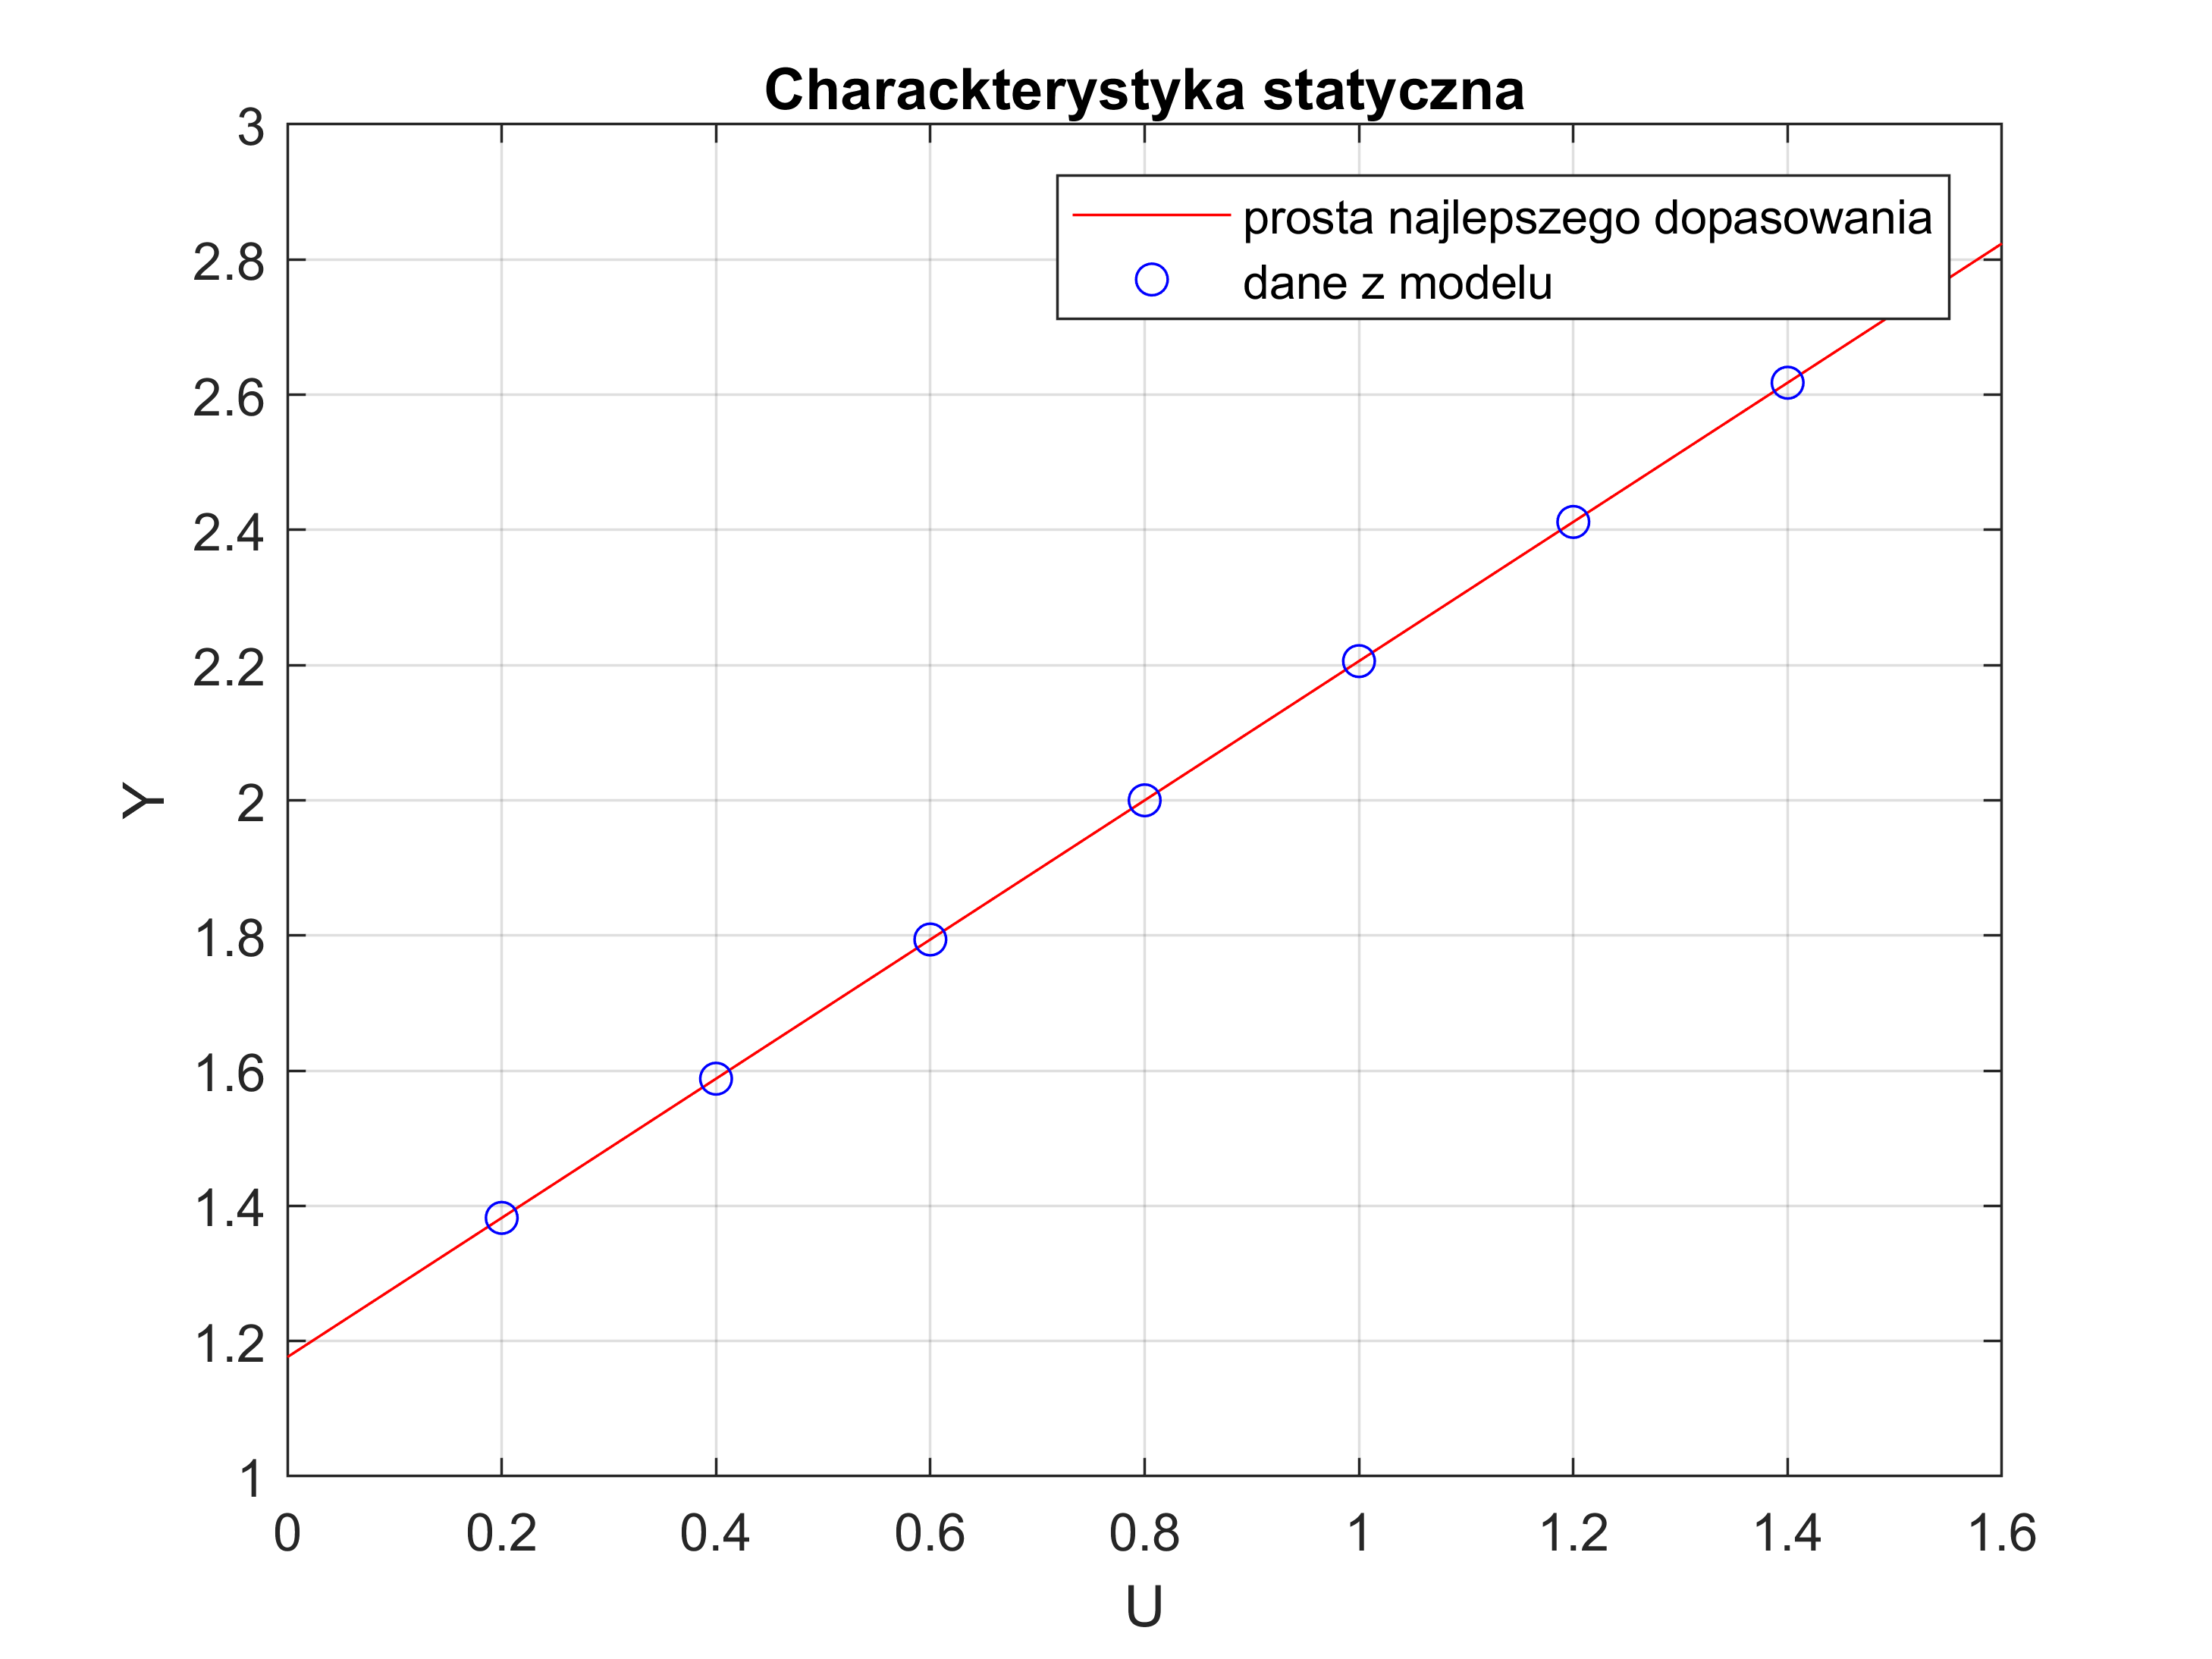
\includegraphics{static_characteristics.png}
\end{figure}

Aby otrzymać odpowiedź skokową wykorzystywaną w algorytmie DMC należy pobudzić obiekt skokiem jednostkowym, gdzie od chwili zerowej sygnał sterujący ma wartość 1, a w przeszłości jest zerowy. Wynik tej odpowiedzi skokowej jest przedstawiony na rys //TODO
\begin{figure}
	//TODO
\end{figure}

\section{Programy do symulacji algorytmów}
Programy do symulacji algorytmów zostały zaimplementowane w plikach \texttt{PID.m} i \texttt{DMC.m}. Funkcje te są wywoływane w każdej kolejnej dyskretnej chwili $k$ i obliczają wartość sterowania jaką należy przesłać na obiekt. Na wejście przyjmują więc obecne wartości zmiennych (PID - uchyb $E$, numer dyskretnej chwili $k$, parametry regulatora dyskretnego $r_{\mathrm{0}}$, $r_{\mathrm{1}}$, $r_{\mathrm{2}}$ i wartość punktu pracy $U_{\mathrm{pp}}$, a DMC dodatkowo jeszcze macierze $K$, $M_{\mathrm{P}}$, wektor $\Delta U_{\mathrm{P}}$). Nakładają one także omówione wcześniej ograniczenia na sygnał sterujący. Funkcje te wywoływane są przez funkcje przeprowadzające symulacje \texttt{PID\_simulation.m} i \texttt{DMC\_simulation.m}, które to z kolei zwracają wartości wyjścia, sterowania i wskaznika jakości i przekazują je do głównego programu.

\section{Ręczny dobór odpowiednich wartości parametrów}
Nastawy regulatora PID i parametry regulatora DMC dobierano metodą eksperymentalną, tj powoli i cierpliwie zmieniając ich wartości oraz obserwując rysunki przedstawiające przebiegi wyjścia procesu. Jak się okazuje optymalnie działający regulator PID przy nastawach ręcznych otrzymaliśmy przy następujących wartościach: $K=\num{0.01}$, $T_\mathrm{i}=10000$, $T_\mathrm{d}=0$, natomiast wskaznik jakości przyjął w tym wypadku wartość $E=\num{122.243}$. Dla algorytmu DMC jakościowo dobre okazały się parametry: $N=50$, $N_\mathrm{u}=1$, $\lambda=\num{1.5}$. Wskaźnik jakości dla tych paramterów przyjął wartość $E=\num{60.614}$  Wyniki symulacji z takimi parametrami znajdują się na rysunkach \ref{dmcinz} oraz ...

\begin{figure}
\label{dmcinz}
\centering
\caption{Przebieg symulacji DMC dla parametrów dobranych metodą eksperymentalną}
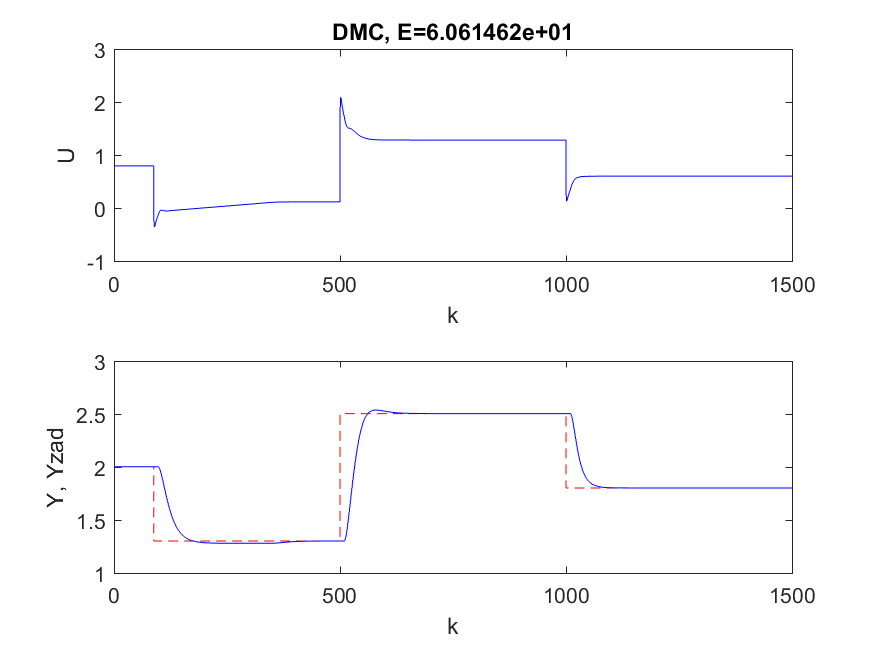
\includegraphics{dmc_inz.png}
\end{figure}

\section{Optymalizacja wskaźnika jakości}
Następnie dokonano optymalizacji wskaźnika jakości regulatorów PID i DMC dla tej samej trajektorii z wykorzystaniem funkcji wbudowanych w środowisku Matlab. Za przyjęty wskaźnik jakości przyjęto sumę kwadratrów róznic pomiędzy wartością zadaną, a wartością wyjścia symulowanego obiektu:

\begin{equation}
E = \sum_{k=1}^{N} (Y^{zad}(k)-Y(k))^2
\end{equation}

Dla regulatora PID do doboru optymalnych parametrów wykorzystano funkcję 
\verb+fmincon+. //TODO: PID do opisania

W przypadku regulatora DMC ze względu na parametry $N$, $N_u$ przyjmujące wartości całkowite należało zastosować funkcję umożliwiającą optymalizację wskaźnika jakości dla parametrów o wartościach całkowitych. W tym celu wykorzystano funkcję \verb+ga+, czyli funkcję wykorzystującą algorytm genetyczny do optymalizacji. W ten sposób otrzymano parametry $N=43$, $N_\mathrm{u}=1$, $\lambda=\num{1.0555}$. Wskaźnik jakości dla tych parametrów wynosi $E=\num{60.369}$. Wyniki symulacji z takimi parametrami znajdują się na rysunkach \ref{dmcopt}

\begin{figure}
\label{dmcopt}
\centering
\caption{Przebieg symulacji DMC dla parametrów dobranych poprzez optymalizację wskaźnika jakości}
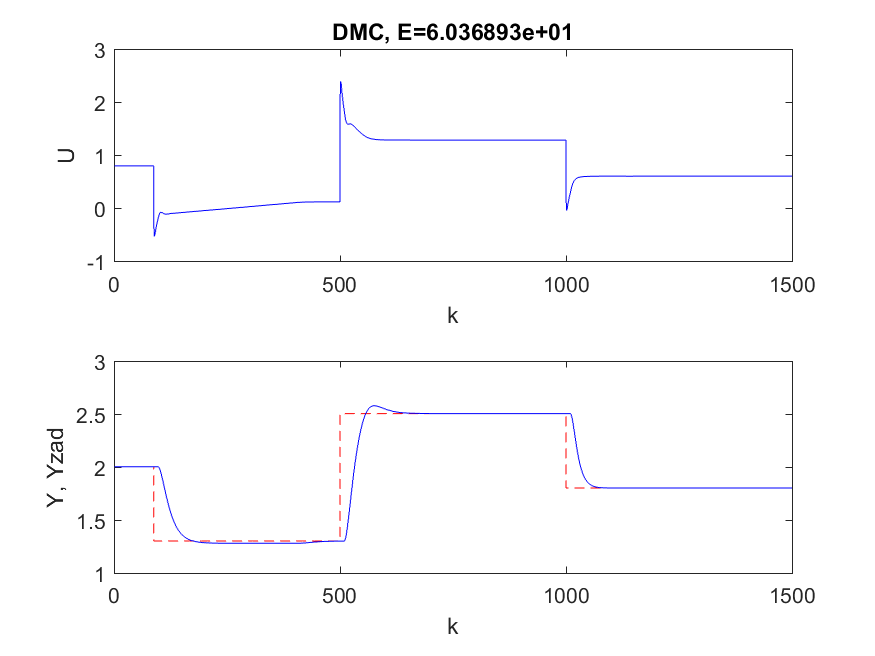
\includegraphics{dmc_optimized.png}
\end{figure}